\documentclass{article}

% content/resources/templates/preamble.tex
\usepackage[margin=0.6in]{geometry}
\author{Milav Dabgar}
\usepackage{amsmath,amssymb,amsthm}
\usepackage{booktabs}
\usepackage{multirow}
\usepackage{xcolor}
\usepackage{tcolorbox}
\tcbuselibrary{breakable,skins}
\usepackage[colorlinks=true,linkcolor=blue]{hyperref}
\usepackage{titlesec}
\usepackage{enumitem}
\usepackage{tikz}
\usepackage{pgfplots}
\usepackage{circuitikz}
\usepackage[version=4]{mhchem}
\usepackage{longtable}
\usepackage{array}
\usepackage{float}
\usepackage{caption}
\usepackage{listings}

\lstset{
  basicstyle=\small\ttfamily,
  breaklines=true,
  breakatwhitespace=false,
  postbreak=\mbox{\textcolor{red}{$\hookrightarrow$}\space},
  float=false,
  numbers=left,
  numberstyle=\tiny\color{gray},
  numbersep=10pt,
  xleftmargin=2em,
  keywordstyle=\color{blue},
  commentstyle=\color{green!60!black},
  stringstyle=\color{purple},
  backgroundcolor=\color{gray!5},
  showstringspaces=false,
  tabsize=2,
  captionpos=b,
  keepspaces=true,
  columns=flexible
}

\pgfplotsset{compat=1.18}
\usetikzlibrary{shapes,arrows,positioning,calc,patterns,decorations.pathmorphing,decorations.markings,arrows.meta}

% Color scheme
\definecolor{headcolor}{RGB}{0,102,204}
\definecolor{keycolor}{RGB}{220,20,60}
\definecolor{solutioncolor}{RGB}{34,139,34}
\definecolor{mnemoniccolor}{RGB}{148,0,211}
\definecolor{codecolor}{RGB}{0,0,100}

% Spacing
\setlength{\parskip}{3pt}
\setlist[itemize]{nosep}
\setlist[enumerate]{nosep}

% Title formatting
\titleformat{\section}{\Large\bfseries\color{headcolor}}{\thesection}{1em}{}
\titleformat{\subsection}{\large\bfseries\color{headcolor}}{\thesubsection}{1em}{}

% Pandoc tightlist compatibility
\providecommand{\tightlist}{%
  \setlength{\itemsep}{0pt}\setlength{\parskip}{0pt}}

% Pandoc longtable compatibility
\newcounter{none}
\def\thenone{}


% content/resources/templates/english-boxes.tex
% This file is currently empty - it exists to maintain consistency with the import structure.
% Add custom environments here if needed in the future.


% Custom commands for GTU solutions
% This file defines semantic commands for consistent formatting

% Question command with automatic formatting
\newcommand{\question}[2]{%
  \section*{Question #1}%
  \textbf{#2}%
}

% OR question variant
\newcommand{\questionor}[2]{%
  \section*{Question #1 OR}%
  \textbf{#2}%
}

% Proper table environment with caption
\newenvironment{answertable}[1]{%
  \begin{table}[htbp]
  \centering
  \caption{#1}
}{%
  \end{table}
}

% Proper figure environment for diagrams
\newenvironment{answerdiagram}[1]{%
  \begin{figure}[htbp]
  \centering
  \caption{#1}
}{%
  \end{figure}
}

% Semantic markup for key terms
\newcommand{\keyword}[1]{\textbf{#1}}
\newcommand{\code}[1]{\texttt{#1}}
\newcommand{\classname}[1]{\texttt{#1}}
\newcommand{\methodname}[1]{\texttt{#1}}

% Proper quotation marks
\newcommand{\mnemonic}[1]{``#1''}

\usetikzlibrary{circuits.ee.IEC}

\title{VLSI (4361102) - Winter 2024 Solution}
\date{November 21, 2024}

\begin{document}
\maketitle

\questionmarks{1}{a}{3}
\textbf{Write advantages of High K FINFET.}

\begin{solutionbox}
    \begin{center}
    \captionof{table}{Advantages of High K FINFET}
    \begin{tabulary}{\linewidth}{L L}
        \hline
        \textbf{Advantage} & \textbf{Description} \\
        \hline
        \textbf{Reduced leakage current} & Better gate control reduces power consumption \\
        \textbf{Improved performance} & Higher drive current and faster switching \\
        \textbf{Better scalability} & Enables continued Moore's law scaling \\
        \hline
    \end{tabulary}
    \end{center}

    \begin{itemize}
        \item \textbf{High K dielectric}: Reduces gate leakage significantly
        \item \textbf{3D structure}: Better electrostatic control over channel
        \item \textbf{Lower power}: Reduced static and dynamic power consumption
    \end{itemize}

    \begin{mnemonicbox}
    High Performance, Low Power, Better Control
    \end{mnemonicbox}
\end{solutionbox}

\questionmarks{1}{b}{4}
\textbf{Define terms: (1) pinch off point (2) Threshold Voltage.}

\begin{solutionbox}
    \begin{center}
    \captionof{table}{Key MOSFET Parameters}
    \begin{tabulary}{\linewidth}{L L L}
        \hline
        \textbf{Term} & \textbf{Definition} & \textbf{Significance} \\
        \hline
        \textbf{Pinch-off Point} & Point where channel becomes completely depleted & Marks transition to saturation region \\
        \textbf{Threshold Voltage} & Minimum $V_{GS}$ needed to form conducting channel & Determines ON/OFF switching point \\
        \hline
    \end{tabulary}
    \end{center}

    \begin{itemize}
        \item \textbf{Pinch-off point}: $V_{DS} = V_{GS} - V_T$, channel narrows to zero width
        \item \textbf{Threshold voltage}: Typically 0.7V for enhancement MOSFET
        \item \textbf{Critical parameters}: Both determine MOSFET operating regions
    \end{itemize}

    \begin{mnemonicbox}
    Threshold Turns ON, Pinch-off Points to Saturation
    \end{mnemonicbox}
\end{solutionbox}

\questionmarks{1}{c}{7}
\textbf{Draw and explain structure of MOSFET transistor.}

\begin{solutionbox}
    \begin{center}
    \captionof{table}{Structure Components}
    \begin{tabulary}{\linewidth}{L L L}
        \hline
        \textbf{Component} & \textbf{Material} & \textbf{Function} \\
        \hline
        \textbf{Gate} & Polysilicon/Metal & Controls channel formation \\
        \textbf{Gate oxide} & SiO2 & Insulates gate from substrate \\
        \textbf{Source/Drain} & n+ doped silicon & Current entry/exit points \\
        \textbf{Substrate} & p-type silicon & Provides body connection \\
        \hline
    \end{tabulary}
    \end{center}

    \begin{center}
    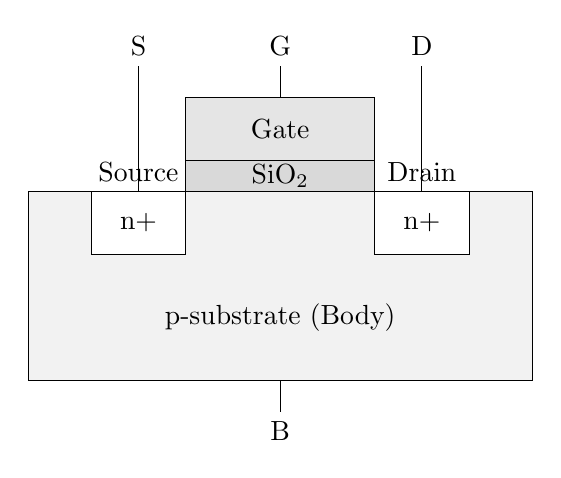
\begin{tikzpicture}[scale=0.8]
        % Substrate
        \draw[fill=gray!10] (0,0) rectangle (8,3);
        \node at (4,1) {p-substrate (Body)};
        
        % Source and Drain Regions
        \draw[fill=white] (1,2) rectangle (2.5,3);
        \node at (1.75,2.5) {n+};
        \node[above] at (1.75,3) {Source};
        
        \draw[fill=white] (5.5,2) rectangle (7,3);
        \node at (6.25,2.5) {n+};
        \node[above] at (6.25,3) {Drain};
        
        % Oxide Layer
        \draw[fill=gray!30] (2.5,3) rectangle (5.5,3.5);
        \node at (4,3.25) {SiO$_2$};
        
        % Gate
        \draw[fill=black!10] (2.5,3.5) rectangle (5.5,4.5);
        \node at (4,4) {Gate};
        
        % Terminals
        \draw (4,4.5) -- (4,5) node[above] {G};
        \draw (1.75,3) -- (1.75,5) node[above] {S};
        \draw (6.25,3) -- (6.25,5) node[above] {D};
        \draw (4,0) -- (4,-0.5) node[below] {B};
    \end{tikzpicture}
    \end{center}

    \begin{itemize}
        \item \textbf{Channel formation}: Occurs at oxide-semiconductor interface
        \item \textbf{Enhancement mode}: Channel forms when $V_{GS} > V_T$
        \item \textbf{Four-terminal device}: Gate, Source, Drain, Body connections
    \end{itemize}

    \begin{mnemonicbox}
    Gate Controls, Oxide Isolates, Source-Drain Conducts
    \end{mnemonicbox}
\end{solutionbox}

\questionmarks{1}{c}{7}
\textbf{Compare Full Voltage Scaling and Constant Voltage Scaling.}

\begin{solutionbox}
    \begin{center}
    \captionof{table}{Full Voltage Scaling vs Constant Voltage Scaling}
    \begin{tabulary}{\linewidth}{L L L}
        \hline
        \textbf{Parameter} & \textbf{Full Voltage Scaling} & \textbf{Constant Voltage Scaling} \\
        \hline
        \textbf{Supply voltage} & Scaled down by $\alpha$ & Remains constant \\
        \textbf{Gate oxide thickness} & Scaled down by $\alpha$ & Scaled down by $\alpha$ \\
        \textbf{Channel length} & Scaled down by $\alpha$ & Scaled down by $\alpha$ \\
        \textbf{Power density} & Remains constant & Increases by $\alpha^2$ \\
        \textbf{Performance} & Moderate improvement & Better performance \\
        \textbf{Reliability} & Better & Degraded due to high fields \\
        \hline
    \end{tabulary}
    \end{center}

    \begin{itemize}
        \item \textbf{Full scaling}: All dimensions and voltages scaled proportionally
        \item \textbf{Constant voltage}: Only physical dimensions scaled, voltage unchanged
        \item \textbf{Trade-off}: Performance vs power vs reliability
    \end{itemize}

    \begin{mnemonicbox}
    Full scales All, Constant keeps Voltage
    \end{mnemonicbox}
\end{solutionbox}

\questionmarks{2}{a}{3}
\textbf{Draw Resistive Load Inverter. Write the input voltage range for different operating region of operation.}

\begin{solutionbox}
    \begin{center}
    \begin{tikzpicture}[circuit ee IEC, font=\sffamily]
        \node [contact] (vdd) at (0,4) {};
        \node [above] at (vdd) {$V_{DD}$};
        \draw (vdd) to [resistor={info={$R_L$}}] (0,2);
        \draw (0,2) -- (1,2) node[right] {$V_{out}$};
        \draw (0,2) -- (0,1.5);
        
        % NMOS
        \node [nmos, xscale=1.5, yscale=1.5] (m1) at (0,0.75) {};
        \node [right] at (m1.east) {M1};
        
        \draw (m1.gate) -- (-1.5, 0.75) node[left] {$V_{in}$};
        \draw (m1.source) -- (0,-0.5) node[ground] {};
        \draw (m1.drain) -- (0,1.5);
    \end{tikzpicture}
    \end{center}

    \begin{center}
    \captionof{table}{Operating Regions}
    \begin{tabulary}{\linewidth}{L L L}
        \hline
        \textbf{Region} & \textbf{Input Voltage Range} & \textbf{Output State} \\
        \hline
        \textbf{Cut-off} & $V_{in} < V_T$ & $V_{out} = V_{DD}$ \\
        \textbf{Triode} & $V_T < V_{in} < V_{DD}-V_T$ & Transition \\
        \textbf{Saturation} & $V_{in} > V_{DD}-V_T$ & $V_{out} \approx 0V$ \\
        \hline
    \end{tabulary}
    \end{center}

    \begin{mnemonicbox}
    Cut-off High, Triode Transition, Saturation Low
    \end{mnemonicbox}
\end{solutionbox}

\questionmarks{2}{b}{4}
\textbf{Draw and Explain VDS-ID and VGS-ID characteristics of N channel MOSFET.}

\begin{solutionbox}
    \begin{center}
    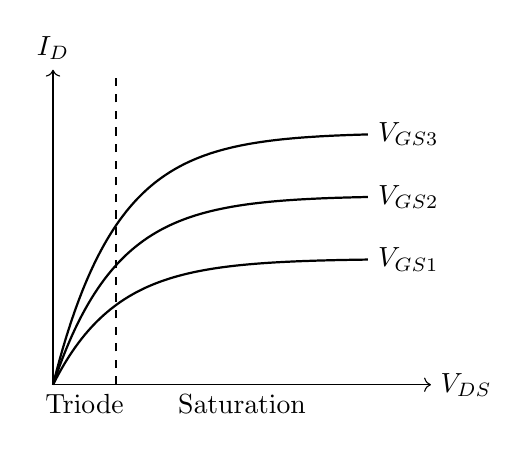
\begin{tikzpicture}[scale=0.8]
        \draw[->] (0,0) -- (6,0) node[right] {$V_{DS}$};
        \draw[->] (0,0) -- (0,5) node[above] {$I_D$};
        
        \draw[thick, domain=0:5, samples=100] plot (\x, {4*(1-exp(-\x))}) node[right] {$V_{GS3}$};
        \draw[thick, domain=0:5, samples=100] plot (\x, {3*(1-exp(-\x))}) node[right] {$V_{GS2}$};
        \draw[thick, domain=0:5, samples=100] plot (\x, {2*(1-exp(-\x))}) node[right] {$V_{GS1}$};
        
        \draw[dashed] (1,0) -- (1,5);
        \node[below] at (0.5,0) {Triode};
        \node[below] at (3,0) {Saturation};
    \end{tikzpicture}
    \end{center}

    \begin{center}
    \captionof{table}{NMOS Characteristics}
    \begin{tabulary}{\linewidth}{L L L}
        \hline
        \textbf{Characteristic} & \textbf{Region} & \textbf{Behavior} \\
        \hline
        \textbf{$V_{DS}-I_D$} & Triode & Linear increase with $V_{DS}$ \\
        \textbf{$V_{DS}-I_D$} & Saturation & Constant $I_D$ (square law) \\
        \textbf{$V_{GS}-I_D$} & Sub-threshold & Exponential increase \\
        \textbf{$V_{GS}-I_D$} & Above $V_T$ & Square law relationship \\
        \hline
    \end{tabulary}
    \end{center}

    \begin{itemize}
        \item \textbf{Triode region}: $I_D$ increases linearly with $V_{DS}$
        \item \textbf{Saturation}: $I_D$ independent of $V_{DS}$, depends on $V_{GS}$
        \item \textbf{Square law}: $I_D \propto (V_{GS}-V_T)^2$ in saturation
    \end{itemize}

    \begin{mnemonicbox}
    Linear in Triode, Square in Saturation
    \end{mnemonicbox}
\end{solutionbox}

\questionmarks{2}{c}{7}
\textbf{Draw \& Explain working of Depletion Load NMOS Inverter circuit.}

\begin{solutionbox}
    \begin{center}
    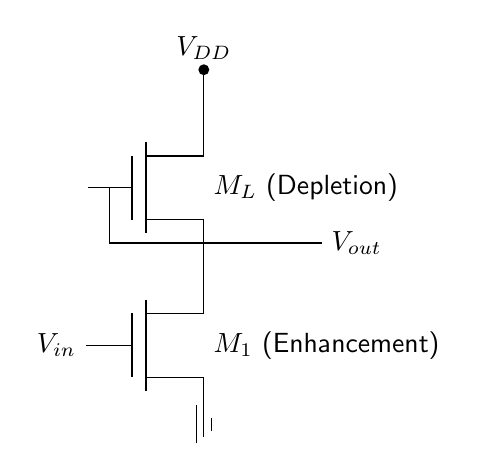
\begin{tikzpicture}[circuit ee IEC, font=\sffamily]
        \node [contact] (vdd) at (0,4) {};
        \node [above] at (vdd) {$V_{DD}$};
        
        % Depletion Load (Simulated with standard symbol + connection)
        \node [nmos, xscale=1.5, yscale=1.5] (ml) at (0,2.5) {};
        \draw (ml.drain) -- (0,4);
        \draw (ml.gate) -- (-1.2, 2.5) -- (-1.2, 1.8) -- (0, 1.8) -- (ml.source); % Gate tied to source
        \node[right] at (ml.east) {$M_L$ (Depletion)};
        
        \draw (0,1.8) -- (1.5,1.8) node[right] {$V_{out}$};
        
        % Driver
        \node [nmos, xscale=1.5, yscale=1.5] (m1) at (0,0.5) {};
        \draw (m1.drain) -- (ml.source);
        \draw (m1.source) -- (0,-0.5) node[ground] {};
        \draw (m1.gate) -- (-1.5, 0.5) node[left] {$V_{in}$};
        \node[right] at (m1.east) {$M_1$ (Enhancement)};
    \end{tikzpicture}
    \end{center}

    \begin{center}
    \captionof{table}{Depletion Load Inverter Operation}
    \begin{tabulary}{\linewidth}{L L L L}
        \hline
        \textbf{Input} & \textbf{M1 State} & \textbf{ML State} & \textbf{Output} \\
        \hline
        \textbf{Low (0V)} & Cut-off & Active load & High ($V_{DD}$) \\
        \textbf{High ($V_{DD}$)} & Saturated & Linear & Low \\
        \hline
    \end{tabulary}
    \end{center}

    \begin{itemize}
        \item \textbf{Depletion load}: Always conducting, acts as current source
        \item \textbf{Better performance}: Higher output voltage swing than resistive load
        \item \textbf{Gate connection}: ML gate tied to source for depletion operation
        \item \textbf{Improved noise margin}: Better $V_{OH}$ compared to enhancement load
    \end{itemize}

    \begin{mnemonicbox}
    Depletion Always ON, Enhancement Controls Flow
    \end{mnemonicbox}
\end{solutionbox}

\questionmarks{2}{a}{3}
\textbf{Describe advantages of CMOS Inverter.}

\begin{solutionbox}
    \begin{center}
    \captionof{table}{Advantages of CMOS Inverter}
    \begin{tabulary}{\linewidth}{L L}
        \hline
        \textbf{Advantage} & \textbf{Benefit} \\
        \hline
        \textbf{Zero static power} & No current in steady state \\
        \textbf{Full voltage swing} & Output swings from 0V to $V_{DD}$ \\
        \textbf{High noise margins} & Better noise immunity \\
        \hline
    \end{tabulary}
    \end{center}

    \begin{itemize}
        \item \textbf{Complementary operation}: One transistor always OFF
        \item \textbf{High input impedance}: Gate isolation provides high impedance
        \item \textbf{Fast switching}: Low parasitic capacitances
    \end{itemize}

    \begin{mnemonicbox}
    Zero Power, Full Swing, High Immunity
    \end{mnemonicbox}
\end{solutionbox}

\questionmarks{2}{b}{4}
\textbf{Draw and Explain Noise Margin in detail.}

\begin{solutionbox}
    \begin{center}
    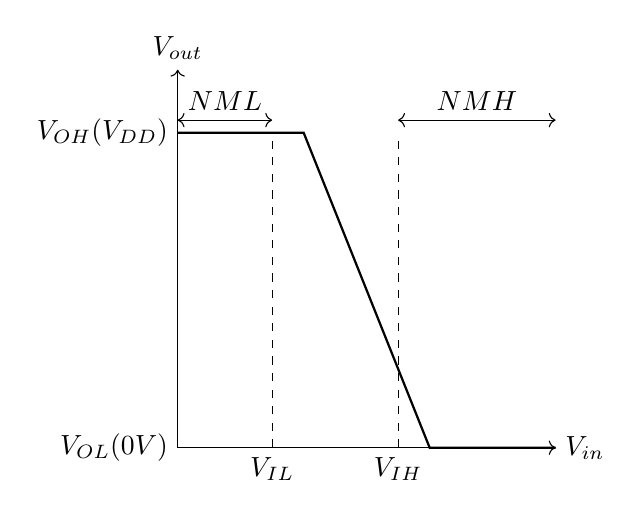
\begin{tikzpicture}[scale=0.8]
        \draw[->] (0,0) -- (6,0) node[right] {$V_{in}$};
        \draw[->] (0,0) -- (0,6) node[above] {$V_{out}$};
        
        \draw[thick] (0,5) -- (2,5) -- (4,0) -- (6,0);
        
        \draw[dashed] (1.5,0) -- (1.5,5);
        \node[below] at (1.5,0) {$V_{IL}$};
        
        \draw[dashed] (3.5,0) -- (3.5,5);
        \node[below] at (3.5,0) {$V_{IH}$};
        
        \node[left] at (0,5) {$V_{OH} (V_{DD})$};
        \node[left] at (0,0) {$V_{OL} (0V)$};
        
        \draw[<->] (0,5.2) -- (1.5,5.2) node[midway, above] {$NML$};
        \draw[<->] (3.5,5.2) -- (6,5.2) node[midway, above] {$NMH$};
    \end{tikzpicture}
    \end{center}

    \begin{center}
    \captionof{table}{Noise Margin Parameters}
    \begin{tabulary}{\linewidth}{L L L}
        \hline
        \textbf{Parameter} & \textbf{Formula} & \textbf{Typical Value} \\
        \hline
        \textbf{$N_{MH}$} & $V_{OH} - V_{IH}$ & 40\% of $V_{DD}$ \\
        \textbf{$N_{ML}$} & $V_{IL} - V_{OL}$ & 40\% of $V_{DD}$ \\
        \hline
    \end{tabulary}
    \end{center}

    \begin{itemize}
        \item \textbf{High noise margin}: Immunity to positive noise
        \item \textbf{Low noise margin}: Immunity to negative noise
        \item \textbf{Better CMOS}: Higher noise margins than other logic families
    \end{itemize}

    \begin{mnemonicbox}
    High goes Higher, Low goes Lower
    \end{mnemonicbox}
\end{solutionbox}

\questionmarks{2}{c}{7}
\textbf{Draw and Explain VTC of N MOS Inverter.}

\begin{solutionbox}
    \begin{center}
    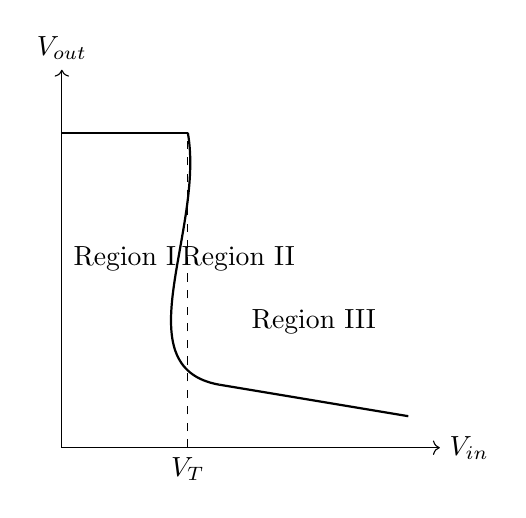
\begin{tikzpicture}[scale=0.8]
        \draw[->] (0,0) -- (6,0) node[right] {$V_{in}$};
        \draw[->] (0,0) -- (0,6) node[above] {$V_{out}$};
        
        % VTC Curve
        \draw[thick] (0,5) -- (2,5); % Cutoff
        \draw[thick] (2,5) to[out=-80, in=170] (2.5,1); % Saturation
        \draw[thick] (2.5,1) -- (5.5,0.5); % Triode
        
        \draw[dashed] (2,0) -- (2,5);
        \node[below] at (2,0) {$V_T$};
        
        \node at (1,3) {Region I};
        \node at (2.8,3) {Region II};
        \node at (4,2) {Region III};
    \end{tikzpicture}
    \end{center}

    \begin{center}
    \captionof{table}{NMOS Inverter Operating Regions}
    \begin{tabulary}{\linewidth}{L L L L}
        \hline
        \textbf{Region} & \textbf{$V_{in}$ Range} & \textbf{M1 State} & \textbf{$V_{out}$} \\
        \hline
        \textbf{I} & 0 to $V_T$ & Cut-off & $V_{DD}$ \\
        \textbf{II} & $V_T$ to $V_T+V_{TL}$ & Saturation & Decreasing \\
        \textbf{III} & $V_T+V_{TL}$ to $V_{DD}$ & Triode & Low \\
        \hline
    \end{tabulary}
    \end{center}

    \begin{itemize}
        \item \textbf{Region I}: M1 OFF, no current flow, $V_{out} = V_{DD}$
        \item \textbf{Region II}: M1 in saturation, sharp transition
        \item \textbf{Region III}: M1 in triode, gradual decrease
        \item \textbf{Load line}: Determines operating point intersection
    \end{itemize}

    \begin{mnemonicbox}
    Cut-off High, Saturation Sharp, Triode Low
    \end{mnemonicbox}
\end{solutionbox}

\questionmarks{3}{a}{3}
\textbf{Draw and explain generalized multiple input NOR gate structure with Depletion NMOS load.}

\begin{solutionbox}
    \begin{center}
    \begin{tikzpicture}[circuit ee IEC, font=\sffamily]
        \node [contact] (vdd) at (0,4) {};
        \node [above] at (vdd) {$V_{DD}$};
        
        % Depletion Load
        \node [nmos, xscale=1.5, yscale=1.5] (ml) at (0,3) {};
        \draw (ml.drain) -- (0,4);
        \draw (ml.gate) -- (-1.2, 3) -- (-1.2, 2.3) -- (0, 2.3) -- (ml.source);
        \node[right] at (ml.east) {$M_L$};
        \draw (0,2.3) -- (2,2.3) node[right] {$Y = (A+B+C)'$};
        
        % Parallel NMOS
        \node [nmos, xscale=1.2, yscale=1.2] (m1) at (-1.5,1) {};
        \node [nmos, xscale=1.2, yscale=1.2] (m2) at (0,1) {};
        \node [nmos, xscale=1.2, yscale=1.2] (m3) at (1.5,1) {};
        
        \draw (0,2.3) -- (0, 1.8) -- (-1.5, 1.8) -- (m1.drain);
        \draw (0,2.3) -- (m2.drain);
        \draw (0,2.3) -- (0, 1.8) -- (1.5, 1.8) -- (m3.drain);
        
        \draw (m1.source) -- (-1.5, 0);
        \draw (m2.source) -- (0, 0);
        \draw (m3.source) -- (1.5, 0);
        \draw (-1.5,0) -- (1.5,0);
        \node [ground] at (0,0) {};
        
        \draw (m1.gate) -- (-2, 1) node[left] {A};
        \draw (m2.gate) -- (-0.5, 1) node[left] {B};
        \draw (m3.gate) -- (1, 1) node[left] {C};
    \end{tikzpicture}
    \end{center}

    \begin{center}
    \captionof{table}{Truth Table for NOR Gate}
    \begin{tabulary}{\linewidth}{L L L}
        \hline
        \textbf{Inputs} & \textbf{Any Input High?} & \textbf{Output Y} \\
        \hline
        \textbf{All Low} & No & High (1) \\
        \textbf{Any High} & Yes & Low (0) \\
        \hline
    \end{tabulary}
    \end{center}

    \begin{itemize}
        \item \textbf{Parallel NMOS}: Any input HIGH pulls output LOW
        \item \textbf{NOR operation}: $Y = (A+B+C)'$
        \item \textbf{Depletion load}: Provides pull-up current
    \end{itemize}

    \begin{mnemonicbox}
    Parallel Pulls Down, Depletion Pulls Up
    \end{mnemonicbox}
\end{solutionbox}

\questionmarks{3}{b}{4}
\textbf{Differentiate AOI and OAI logic circuits.}

\begin{solutionbox}
    \begin{center}
    \captionof{table}{AOI vs OAI Logic}
    \begin{tabulary}{\linewidth}{L L L}
        \hline
        \textbf{Parameter} & \textbf{AOI (AND-OR-Invert)} & \textbf{OAI (OR-AND-Invert)} \\
        \hline
        \textbf{Logic function} & $Y = (AB + CD)'$ & $Y = ((A+B)(C+D))'$ \\
        \textbf{NMOS structure} & Series-parallel & Parallel-series \\
        \textbf{PMOS structure} & Parallel-series & Series-parallel \\
        \textbf{Complexity} & Moderate & Moderate \\
        \hline
    \end{tabulary}
    \end{center}

    \begin{itemize}
        \item \textbf{AOI}: AND terms ORed then inverted
        \item \textbf{OAI}: OR terms ANDed then inverted
        \item \textbf{CMOS implementation}: Dual network structure
        \item \textbf{Applications}: Complex logic functions in single stage
    \end{itemize}

    \begin{mnemonicbox}
    AOI: AND-OR-Invert, OAI: OR-AND-Invert
    \end{mnemonicbox}
\end{solutionbox}

\questionmarks{3}{c}{7}
\textbf{Implement two input EX-OR gate using CMOS, and logic function Z = (AB +CD)' using NMOS Load.}

\begin{solutionbox}
    \textbf{EX-OR CMOS Implementation:}
    \begin{center}
    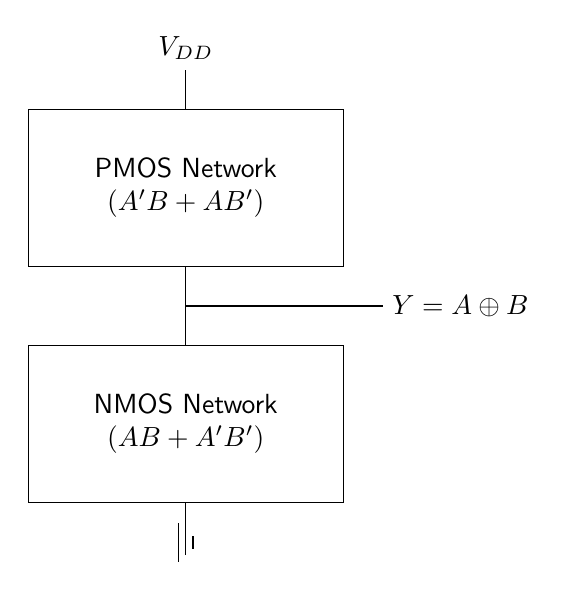
\begin{tikzpicture}[circuit ee IEC, font=\sffamily]
        % Abstract Block Diagram for Complexity
        \draw (0,0) rectangle (4,2);
        \node[align=center] at (2,1) {PMOS Network\\$(A'B + AB')$};
        
        \draw (0,-3) rectangle (4,-1);
        \node[align=center] at (2,-2) {NMOS Network\\$(AB + A'B')$};
        
        \draw (2,2) -- (2,2.5) node[above] {$V_{DD}$};
        \draw (2,-3) -- (2,-3.5) node[ground] {};
        \draw (2,0) -- (2,-1);
        \draw (2,-0.5) -- (4.5,-0.5) node[right] {$Y = A \oplus B$};
    \end{tikzpicture}
    \end{center}

    \textbf{Z = (AB + CD)' NMOS Implementation:}
    \begin{center}
    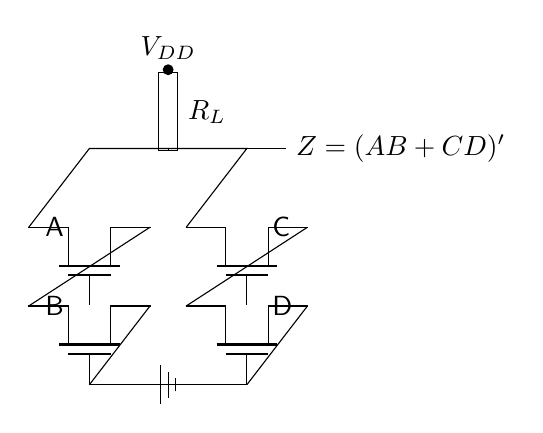
\begin{tikzpicture}[circuit ee IEC, font=\sffamily]
        \node [contact] (vdd) at (2,4) {};
        \node [above] at (vdd) {$V_{DD}$};
        \draw (vdd) to [resistor={info={$R_L$}}] (2,3);
        \draw (2,3) -- (3.5,3) node[right] {$Z = (AB + CD)'$};
        
        % NMOS Series AB
        \node [nmos, rotate=90] (m1) at (1,2) {}; % A
        \node [nmos, rotate=90] (m2) at (1,1) {}; % B
        \draw (2,3) -- (1,3) -- (m1.drain);
        \draw (m1.source) -- (m2.drain);
        \draw (m2.source) -- (1,0); 
        
        % NMOS Series CD
        \node [nmos, rotate=90] (m3) at (3,2) {}; % C
        \node [nmos, rotate=90] (m4) at (3,1) {}; % D
        \draw (2,3) -- (3,3) -- (m3.drain);
        \draw (m3.source) -- (m4.drain);
        \draw (m4.source) -- (3,0);
        
        \draw (1,0) -- (3,0);
        \node [ground] at (2,0) {};
        
        \node [left] at (0.8, 2) {A};
        \node [left] at (0.8, 1) {B};
        \node [right] at (3.2, 2) {C};
        \node [right] at (3.2, 1) {D};
    \end{tikzpicture}
    \end{center}

    \begin{center}
    \captionof{table}{Logic Implementation Comparison}
    \begin{tabulary}{\linewidth}{L L L}
        \hline
        \textbf{Circuit} & \textbf{Function} & \textbf{Implementation} \\
        \hline
        \textbf{EX-OR} & $A \oplus B$ & Complementary CMOS \\
        \textbf{AOI} & $(AB+CD)'$ & Series-parallel NMOS \\
        \hline
    \end{tabulary}
    \end{center}

    \begin{itemize}
        \item \textbf{EX-OR}: Requires transmission gates for efficient implementation
        \item \textbf{AOI function}: Natural NMOS implementation
        \item \textbf{Power consideration}: CMOS has zero static power
    \end{itemize}

    \begin{mnemonicbox}
    EX-OR needs Transmission, AOI uses Series-Parallel
    \end{mnemonicbox}
\end{solutionbox}

\questionmarks{3}{a}{3}
\textbf{Draw and explain generalized multiple input NAND gate structure with Depletion NMOS load.}

\begin{solutionbox}
    \begin{center}
    \begin{tikzpicture}[circuit ee IEC, font=\sffamily]
        \node [contact] (vdd) at (0,4.5) {};
        \node [above] at (vdd) {$V_{DD}$};
        
        % Depletion Load
        \node [nmos, xscale=1.5, yscale=1.5] (ml) at (0,3.5) {};
        \draw (ml.drain) -- (0,4.5);
        \draw (ml.gate) -- (-1.2, 3.5) -- (-1.2, 2.8) -- (0, 2.8) -- (ml.source);
        \node[right] at (ml.east) {$M_L$};
        \draw (0,2.8) -- (1.5,2.8) node[right] {$Y = (ABC)'$};
        
        % Series NMOS
        \node [nmos, xscale=1.2, yscale=1.2] (m1) at (0,2) {};
        \node [nmos, xscale=1.2, yscale=1.2] (m2) at (0,0.8) {};
        \node [nmos, xscale=1.2, yscale=1.2] (m3) at (0,-0.4) {};
        
        \draw (0,2.8) -- (m1.drain);
        \draw (m1.source) -- (m2.drain);
        \draw (m2.source) -- (m3.drain);
        \draw (m3.source) -- (0,-1) node[ground] {};
        
        \draw (m1.gate) -- (-1, 2) node[left] {A};
        \draw (m2.gate) -- (-1, 0.8) node[left] {B};
        \draw (m3.gate) -- (-1, -0.4) node[left] {C};
    \end{tikzpicture}
    \end{center}

    \begin{center}
    \captionof{table}{NAND Gate Operation}
    \begin{tabulary}{\linewidth}{L L L}
        \hline
        \textbf{Condition} & \textbf{Path to Ground} & \textbf{Output Y} \\
        \hline
        \textbf{All inputs HIGH} & Complete path & Low (0) \\
        \textbf{Any input LOW} & Broken path & High (1) \\
        \hline
    \end{tabulary}
    \end{center}

    \begin{itemize}
        \item \textbf{Series NMOS}: All inputs must be HIGH to pull output LOW
        \item \textbf{NAND operation}: $Y = (ABC)'$
        \item \textbf{Depletion load}: Always provides pull-up current
    \end{itemize}

    \begin{mnemonicbox}
    Series Needs All, NAND Says Not-AND
    \end{mnemonicbox}
\end{solutionbox}

\questionmarks{3}{b}{4}
\textbf{Implement logic function Y = ((P+R)(S+T))' using CMOS logic.}

\begin{solutionbox}
    \begin{center}
    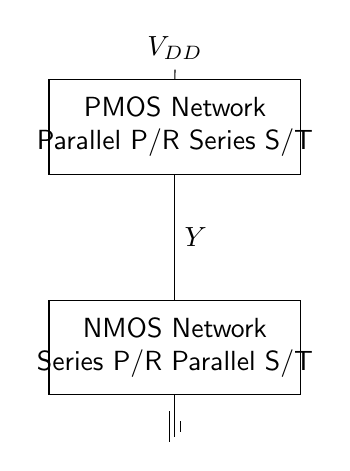
\begin{tikzpicture}[circuit ee IEC, font=\sffamily, scale=0.8]
        \node (vdd) at (2,6) {$V_{DD}$};
        \draw (0,4) rectangle (4,5.5);
        \node[align=center] at (2,4.75) {PMOS Network\\Parallel P/R Series S/T};
        
        \draw (2,5.5) -- (vdd);
        \draw (2,4) -- (2,3) node[right] {$Y$};
        
        \draw (0,0.5) rectangle (4,2);
        \node[align=center] at (2,1.25) {NMOS Network\\Series P/R Parallel S/T};
        \draw (2,3) -- (2,2);
        \draw (2,0.5) -- (2,0) node[ground] {};
    \end{tikzpicture}
    \end{center}

    \begin{center}
    \captionof{table}{Truth Table Implementation}
    \begin{tabulary}{\linewidth}{L L L}
        \hline
        \textbf{PMOS Network} & \textbf{NMOS Network} & \textbf{Operation} \\
        \hline
        \textbf{$(P+R)'+(S+T)'$} & \textbf{$(P+R)(S+T)$} & Complementary \\
        \textbf{$P'R' + S'T'$} & \textbf{$PS + PT + RS + RT$} & De Morgan's law \\
        \hline
    \end{tabulary}
    \end{center}

    \begin{itemize}
        \item \textbf{PMOS}: Parallel within groups, series between groups
        \item \textbf{NMOS}: Series within groups, parallel between groups
        \item \textbf{Dual network}: Ensures complementary operation
    \end{itemize}

    \begin{mnemonicbox}
    PMOS does Opposite of NMOS
    \end{mnemonicbox}
\end{solutionbox}

\questionmarks{3}{c}{7}
\textbf{Describe the working of SR latch circuit.}

\begin{solutionbox}
    \begin{center}
    \begin{tikzpicture}
        \node[gtu block] (nor1) at (0,1.5) {NOR 1};
        \node[gtu block] (nor2) at (0,-1.5) {NOR 2};
        
        \draw[->] (-2,1.7) node[left]{S} -- (nor1.160);
        \draw[->] (-2,-1.7) node[left]{R} -- (nor2.200);
        
        \draw[->] (nor1.0) -- (2,1.5) node[right]{Q};
        \draw[->] (nor2.0) -- (2,-1.5) node[right]{Q'};
        
        % Feedback
        \draw (nor1.0) -- (0.5,1.5) -- (0.5,0.5) -- (-1,-0.5) -- (-1,-1.3) -- (nor2.160);
        \draw (nor2.0) -- (0.5,-1.5) -- (0.5,-0.5) -- (-1,0.5) -- (-1,1.3) -- (nor1.200);
    \end{tikzpicture}
    \end{center}

    \begin{center}
    \captionof{table}{SR Latch Truth Table}
    \begin{tabulary}{\linewidth}{L L L L L}
        \hline
        \textbf{S} & \textbf{R} & \textbf{Q(n+1)} & \textbf{Q'(n+1)} & \textbf{State} \\
        \hline
        \textbf{0} & \textbf{0} & Q(n) & Q'(n) & Hold \\
        \textbf{0} & \textbf{1} & 0 & 1 & Reset \\
        \textbf{1} & \textbf{0} & 1 & 0 & Set \\
        \textbf{1} & \textbf{1} & 0 & 0 & Invalid \\
        \hline
    \end{tabulary}
    \end{center}

    \begin{itemize}
        \item \textbf{Set operation}: S=1, R=0 makes Q=1
        \item \textbf{Reset operation}: S=0, R=1 makes Q=0
        \item \textbf{Hold state}: S=0, R=0 maintains previous state
        \item \textbf{Invalid state}: S=1, R=1 should be avoided
        \item \textbf{Cross-coupled}: Output of one gate feeds input of other
    \end{itemize}

    \begin{mnemonicbox}
    Set Sets, Reset Resets, Both Bad
    \end{mnemonicbox}
\end{solutionbox}

\questionmarks{4}{a}{3}
\textbf{Compare Etching methods in chip fabrication.}

\begin{solutionbox}
    \begin{center}
    \captionof{table}{Etching Methods Comparison}
    \begin{tabulary}{\linewidth}{L L L L}
        \hline
        \textbf{Method} & \textbf{Type} & \textbf{Advantages} & \textbf{Disadvantages} \\
        \hline
        \textbf{Wet Etching} & Chemical & High selectivity, simple & Isotropic, undercut \\
        \textbf{Dry Etching} & Physical/Chemical & Anisotropic, precise & Complex equipment \\
        \textbf{Plasma Etching} & Ion bombardment & Directional control & Damage to surface \\
        \hline
    \end{tabulary}
    \end{center}

    \begin{itemize}
        \item \textbf{Wet etching}: Uses liquid chemicals, attacks all directions
        \item \textbf{Dry etching}: Uses gases/plasma, better directional control
        \item \textbf{Selectivity}: Ability to etch one material over another
    \end{itemize}

    \begin{mnemonicbox}
    Wet is Wide, Dry is Directional
    \end{mnemonicbox}
\end{solutionbox}

\questionmarks{4}{b}{4}
\textbf{Write short note on Lithography.}

\begin{solutionbox}
    \begin{center}
    \captionof{table}{Lithography Process Steps}
    \begin{tabulary}{\linewidth}{L L L}
        \hline
        \textbf{Step} & \textbf{Process} & \textbf{Purpose} \\
        \hline
        \textbf{Resist coating} & Spin-on photoresist & Light-sensitive layer \\
        \textbf{Exposure} & UV light through mask & Pattern transfer \\
        \textbf{Development} & Remove exposed resist & Reveal pattern \\
        \textbf{Etching} & Remove unprotected material & Create features \\
        \hline
    \end{tabulary}
    \end{center}

    \begin{itemize}
        \item \textbf{Pattern transfer}: From mask to silicon wafer
        \item \textbf{Resolution}: Determines minimum feature size
        \item \textbf{Alignment}: Critical for multiple layer processing
        \item \textbf{UV wavelength}: Shorter wavelength gives better resolution
    \end{itemize}

    \begin{mnemonicbox}
    Coat, Expose, Develop, Etch
    \end{mnemonicbox}
\end{solutionbox}

\questionmarks{4}{c}{7}
\textbf{Explain Regularity, Modularity and Locality.}

\begin{solutionbox}
    \begin{center}
    \captionof{table}{Design Principles}
    \begin{tabulary}{\linewidth}{L L L L}
        \hline
        \textbf{Principle} & \textbf{Definition} & \textbf{Benefits} & \textbf{Example} \\
        \hline
        \textbf{Regularity} & Repeated identical structures & Easier design, testing & Memory arrays \\
        \textbf{Modularity} & Hierarchical design blocks & Reusability, maintainability & Standard cells \\
        \textbf{Locality} & Related functions grouped & Reduced interconnect & Functional blocks \\
        \hline
    \end{tabulary}
    \end{center}

    \textbf{Implementation Details:}
    \begin{itemize}
        \item \textbf{Regularity}: Same cell repeated multiple times reduces design complexity
        \item \textbf{Modularity}: Top-down design with well-defined interfaces
        \item \textbf{Locality}: Minimizes wire delays and routing congestion
        \item \textbf{Design benefits}: Faster design cycle, better testability
        \item \textbf{Manufacturing}: Improved yield through regular patterns
    \end{itemize}

    \begin{center}
    \begin{tikzpicture}
        \node[gtu block] (sys) at (0,0) {System Level};
        \node[gtu block, right=of sys] (mod) {Module Level};
        \node[gtu block, right=of mod] (cell) {Cell Level};
        \node[gtu block, right=of cell] (dev) {Device Level};
        
        \path[gtu arrow] (sys) edge (mod);
        \path[gtu arrow] (mod) edge (cell);
        \path[gtu arrow] (cell) edge (dev);
    \end{tikzpicture}
    \end{center}

    \begin{mnemonicbox}
    Regular Modules with Local Connections
    \end{mnemonicbox}
\end{solutionbox}

\questionmarks{4}{a}{3}
\textbf{Define Design Hierarchy.}

\begin{solutionbox}
    \begin{center}
    \captionof{table}{Design Hierarchy Levels}
    \begin{tabulary}{\linewidth}{L L L}
        \hline
        \textbf{Level} & \textbf{Description} & \textbf{Components} \\
        \hline
        \textbf{System} & Complete chip functionality & Processors, memories \\
        \textbf{Module} & Major functional blocks & ALU, cache, I/O \\
        \textbf{Cell} & Basic logic elements & Gates, flip-flops \\
        \hline
    \end{tabulary}
    \end{center}

    \begin{itemize}
        \item \textbf{Top-down approach}: System broken into smaller modules
        \item \textbf{Abstraction levels}: Each level hides lower level details
        \item \textbf{Interface definition}: Clear boundaries between levels
    \end{itemize}

    \begin{mnemonicbox}
    System to Module to Cell
    \end{mnemonicbox}
\end{solutionbox}

\questionmarks{4}{b}{4}
\textbf{Draw and Explain VLSI design flow chart.}

\begin{solutionbox}
    \begin{center}
    \begin{tikzpicture}[node distance=1.5cm, auto]
        \node[gtu block] (spec) {System Specification};
        \node[gtu block, below=of spec] (arch) {Architectural Design};
        \node[gtu block, below=of arch] (logic) {Logic Design};
        \node[gtu block, below=of logic] (circ) {Circuit Design};
        \node[gtu block, below=of circ] (lay) {Layout Design};
        \node[gtu block, below=of lay] (fab) {Fabrication};
        \node[gtu block, below=of fab] (test) {Testing};
        
        \path[gtu arrow] (spec) edge (arch);
        \path[gtu arrow] (arch) edge (logic);
        \path[gtu arrow] (logic) edge (circ);
        \path[gtu arrow] (circ) edge (lay);
        \path[gtu arrow] (lay) edge (fab);
        \path[gtu arrow] (fab) edge (test);
    \end{tikzpicture}
    \end{center}

    \begin{center}
    \captionof{table}{Design Flow Stages}
    \begin{tabulary}{\linewidth}{L L L L}
        \hline
        \textbf{Stage} & \textbf{Input} & \textbf{Output} & \textbf{Tools} \\
        \hline
        \textbf{Architecture} & Specifications & Block diagram & High-level modeling \\
        \textbf{Logic} & Architecture & Gate netlist & HDL synthesis \\
        \textbf{Circuit} & Netlist & Transistor sizing & SPICE simulation \\
        \textbf{Layout} & Circuit & Mask data & Place \& route \\
        \hline
    \end{tabulary}
    \end{center}

    \begin{mnemonicbox}
    Specify, Architect, Logic, Circuit, Layout, Fabricate, Test
    \end{mnemonicbox}
\end{solutionbox}

\questionmarks{4}{c}{7}
\textbf{Write short note on 'VLSI Fabrication Process'}

\begin{solutionbox}
    \begin{center}
    \captionof{table}{Major Fabrication Steps}
    \begin{tabulary}{\linewidth}{L L L}
        \hline
        \textbf{Process} & \textbf{Purpose} & \textbf{Result} \\
        \hline
        \textbf{Oxidation} & Grow SiO2 layer & Gate oxide formation \\
        \textbf{Lithography} & Pattern transfer & Define device areas \\
        \textbf{Etching} & Remove unwanted material & Create device structures \\
        \textbf{Ion Implantation} & Add dopants & Create P/N regions \\
        \textbf{Deposition} & Add material layers & Metal interconnects \\
        \textbf{Diffusion} & Spread dopants & Junction formation \\
        \hline
    \end{tabulary}
    \end{center}

    \textbf{Process Flow:}
    \begin{itemize}
        \item \textbf{Wafer preparation}: Clean silicon substrate
        \item \textbf{Device formation}: Create transistors through multiple steps
        \item \textbf{Interconnect}: Add metal layers for connections
        \item \textbf{Passivation}: Protect completed circuit
        \item \textbf{Testing}: Verify functionality before packaging
    \end{itemize}

    \textbf{Clean Room Requirements:}
    \begin{itemize}
        \item \textbf{Class 1-10}: Ultra-clean environment needed
        \item \textbf{Temperature control}: Precise process control
        \item \textbf{Chemical purity}: High-grade materials required
    \end{itemize}

    \begin{mnemonicbox}
    Oxidize, Pattern, Etch, Implant, Deposit, Diffuse
    \end{mnemonicbox}
\end{solutionbox}

\questionmarks{5}{a}{3}
\textbf{Compare different styles of Verilog programming in VLSI.}

\begin{solutionbox}
    \begin{center}
    \captionof{table}{Verilog Modeling Styles}
    \begin{tabulary}{\linewidth}{L L L}
        \hline
        \textbf{Style} & \textbf{Description} & \textbf{Application} \\
        \hline
        \textbf{Behavioral} & Algorithm description & High-level modeling \\
        \textbf{Dataflow} & Boolean expressions & Combinational logic \\
        \textbf{Structural} & Gate-level description & Hardware representation \\
        \hline
    \end{tabulary}
    \end{center}

    \begin{itemize}
        \item \textbf{Behavioral}: Uses always blocks, if-else, case statements
        \item \textbf{Dataflow}: Uses assign statements with Boolean operators
        \item \textbf{Structural}: Instantiates gates and modules explicitly
    \end{itemize}

    \begin{mnemonicbox}
    Behavior Describes, Dataflow Assigns, Structure Connects
    \end{mnemonicbox}
\end{solutionbox}

\questionmarks{5}{b}{4}
\textbf{Write Verilog program of NAND gate using behavioral method.}

\begin{solutionbox}
\begin{lstlisting}[language=Verilog]
module nand_gate_behavioral(
    input wire a, b,
    output reg y
);

always @(a or b) begin
    if (a == 1'b1 && b == 1'b1)
        y = 1'b0;
    else
        y = 1'b1;
end

endmodule
\end{lstlisting}

    \textbf{Code Explanation:}
    \begin{itemize}
        \item \textbf{Always block}: Executes when inputs change
        \item \textbf{Sensitivity list}: Contains all input signals
        \item \textbf{Conditional statement}: Implements NAND logic
        \item \textbf{Reg declaration}: Required for procedural assignment
    \end{itemize}

    \begin{mnemonicbox}
    Always watch, IF both high THEN low ELSE high
    \end{mnemonicbox}
\end{solutionbox}

\questionmarks{5}{c}{7}
\textbf{Draw 4X1 multiplexer circuit. Develop Verilog program of the circuit using case statement.}

\begin{solutionbox}
    \textbf{4X1 Multiplexer Circuit:}
    \begin{center}
    \begin{tikzpicture}
        \node[draw, minimum width=2cm, minimum height=3cm] (mux) {MUX 4X1};
        
        \draw[<-] (mux.160) -- +(-1,0) node[left] {$I_0$};
        \draw[<-] (mux.170) -- +(-1,0) node[left] {$I_1$};
        \draw[<-] (mux.190) -- +(-1,0) node[left] {$I_2$};
        \draw[<-] (mux.200) -- +(-1,0) node[left] {$I_3$};
        
        \draw[->] (mux.0) -- +(1,0) node[right] {$Y$};
        
        \draw[<-] (mux.270) -- +(0,-1) node[below] {$S_1, S_0$};
    \end{tikzpicture}
    \end{center}

    \textbf{Verilog Code:}
\begin{lstlisting}[language=Verilog]
module mux_4x1_case(
    input wire [1:0] sel,
    input wire i0, i1, i2, i3,
    output reg y
);

always @(*) begin
    case (sel)
        2'b00: y = i0;
        2'b01: y = i1;
        2'b10: y = i2;
        2'b11: y = i3;
        default: y = 1'bx;
    endcase
end

endmodule
\end{lstlisting}

    \begin{center}
    \captionof{table}{MUX Truth Table}
    \begin{tabulary}{\linewidth}{L L L}
        \hline
        \textbf{S1} & \textbf{S0} & \textbf{Output Y} \\
        \hline
        \textbf{0} & \textbf{0} & I0 \\
        \textbf{0} & \textbf{1} & I1 \\
        \textbf{1} & \textbf{0} & I2 \\
        \textbf{1} & \textbf{1} & I3 \\
        \hline
    \end{tabulary}
    \end{center}

    \begin{mnemonicbox}
    Case Selects, Default Protects
    \end{mnemonicbox}
\end{solutionbox}

\questionmarks{5}{a}{3}
\textbf{Define Testbench with example.}

\begin{solutionbox}
    \textbf{Testbench Definition:}
    Testbench is a Verilog module that provides stimulus to design under test (DUT) and monitors its response.

    \textbf{Example Testbench:}
\begin{lstlisting}[language=Verilog]
module test_and_gate;
    reg a, b;
    wire y;
    
    and_gate dut(.a(a), .b(b), .y(y));
    
    initial begin
        a = 0; b = 0; #10;
        a = 0; b = 1; #10;
        a = 1; b = 0; #10;
        a = 1; b = 1; #10;
    end
endmodule
\end{lstlisting}

    \begin{itemize}
        \item \textbf{DUT instantiation}: Creates instance of design under test
        \item \textbf{Stimulus generation}: Provides input test vectors
        \item \textbf{No ports}: Testbench is top-level module
    \end{itemize}

    \begin{mnemonicbox}
    Test Provides Stimulus, Monitors Response
    \end{mnemonicbox}
\end{solutionbox}

\questionmarks{5}{b}{4}
\textbf{Write Verilog program of Half Adder using Dataflow method.}

\begin{solutionbox}
\begin{lstlisting}[language=Verilog]
module half_adder_dataflow(
    input wire a, b,
    output wire sum, carry
);

assign sum = a ^ b;    // XOR for sum
assign carry = a & b;  // AND for carry

endmodule
\end{lstlisting}

    \textbf{Logic Implementation:}
    \begin{itemize}
        \item \textbf{Sum}: XOR operation between inputs
        \item \textbf{Carry}: AND operation between inputs
        \item \textbf{Assign statement}: Continuous assignment for dataflow
        \item \textbf{Boolean operators}: \^{} (XOR), \& (AND)
    \end{itemize}

    \begin{center}
    \captionof{table}{Half Adder Truth Table}
    \begin{tabulary}{\linewidth}{L L L L}
        \hline
        \textbf{A} & \textbf{B} & \textbf{Sum} & \textbf{Carry} \\
        \hline
        \textbf{0} & \textbf{0} & 0 & 0 \\
        \textbf{0} & \textbf{1} & 1 & 0 \\
        \textbf{1} & \textbf{0} & 1 & 0 \\
        \textbf{1} & \textbf{1} & 0 & 1 \\
        \hline
    \end{tabulary}
    \end{center}

    \begin{mnemonicbox}
    XOR Sums, AND Carries
    \end{mnemonicbox}
\end{solutionbox}

\questionmarks{5}{c}{7}
\textbf{Write function of Encoder. Develop code of 8X3 Encoder using if….else statement.}

\begin{solutionbox}
    \textbf{Encoder Function:}
    Encoder converts $2^n$ input lines to $n$ output lines. 8X3 encoder converts 8 inputs to 3-bit binary output.

    \textbf{Priority Table:}
    \begin{tabulary}{\linewidth}{L L}
        \hline
        \textbf{Input} & \textbf{Binary Output} \\
        \hline
        \textbf{I7} & 111 \\
        \textbf{I6} & 110 \\
        \textbf{I5} & 101 \\
        \textbf{I4} & 100 \\
        \textbf{I3} & 011 \\
        \textbf{I2} & 010 \\
        \textbf{I1} & 001 \\
        \textbf{I0} & 000 \\
        \hline
    \end{tabulary}

    \textbf{Verilog Code:}
\begin{lstlisting}[language=Verilog]
module encoder_8x3(
    input wire [7:0] i,
    output reg [2:0] y
);

always @(*) begin
    if (i[7])
        y = 3'b111;
    else if (i[6])
        y = 3'b110;
    else if (i[5])
        y = 3'b101;
    else if (i[4])
        y = 3'b100;
    else if (i[3])
        y = 3'b011;
    else if (i[2])
        y = 3'b010;
    else if (i[1])
        y = 3'b001;
    else if (i[0])
        y = 3'b000;
    else
        y = 3'bxxx;
end

endmodule
\end{lstlisting}

    \begin{itemize}
        \item \textbf{Priority encoding}: Higher index inputs have priority
        \item \textbf{If-else chain}: Implements priority logic
        \item \textbf{Binary encoding}: Converts active input to binary representation
    \end{itemize}

    \begin{mnemonicbox}
    Priority from High to Low, Binary Output Flows
    \end{mnemonicbox}
\end{solutionbox}

\end{document}
